% ============================================================
% SECTION 4 — DEMO MODEL
% ============================================================

\section{Demo Model}

% Slide 1 — ART Retrieval Workflow
\begin{frame}{Quy trình truy hồi của ART}

\centering
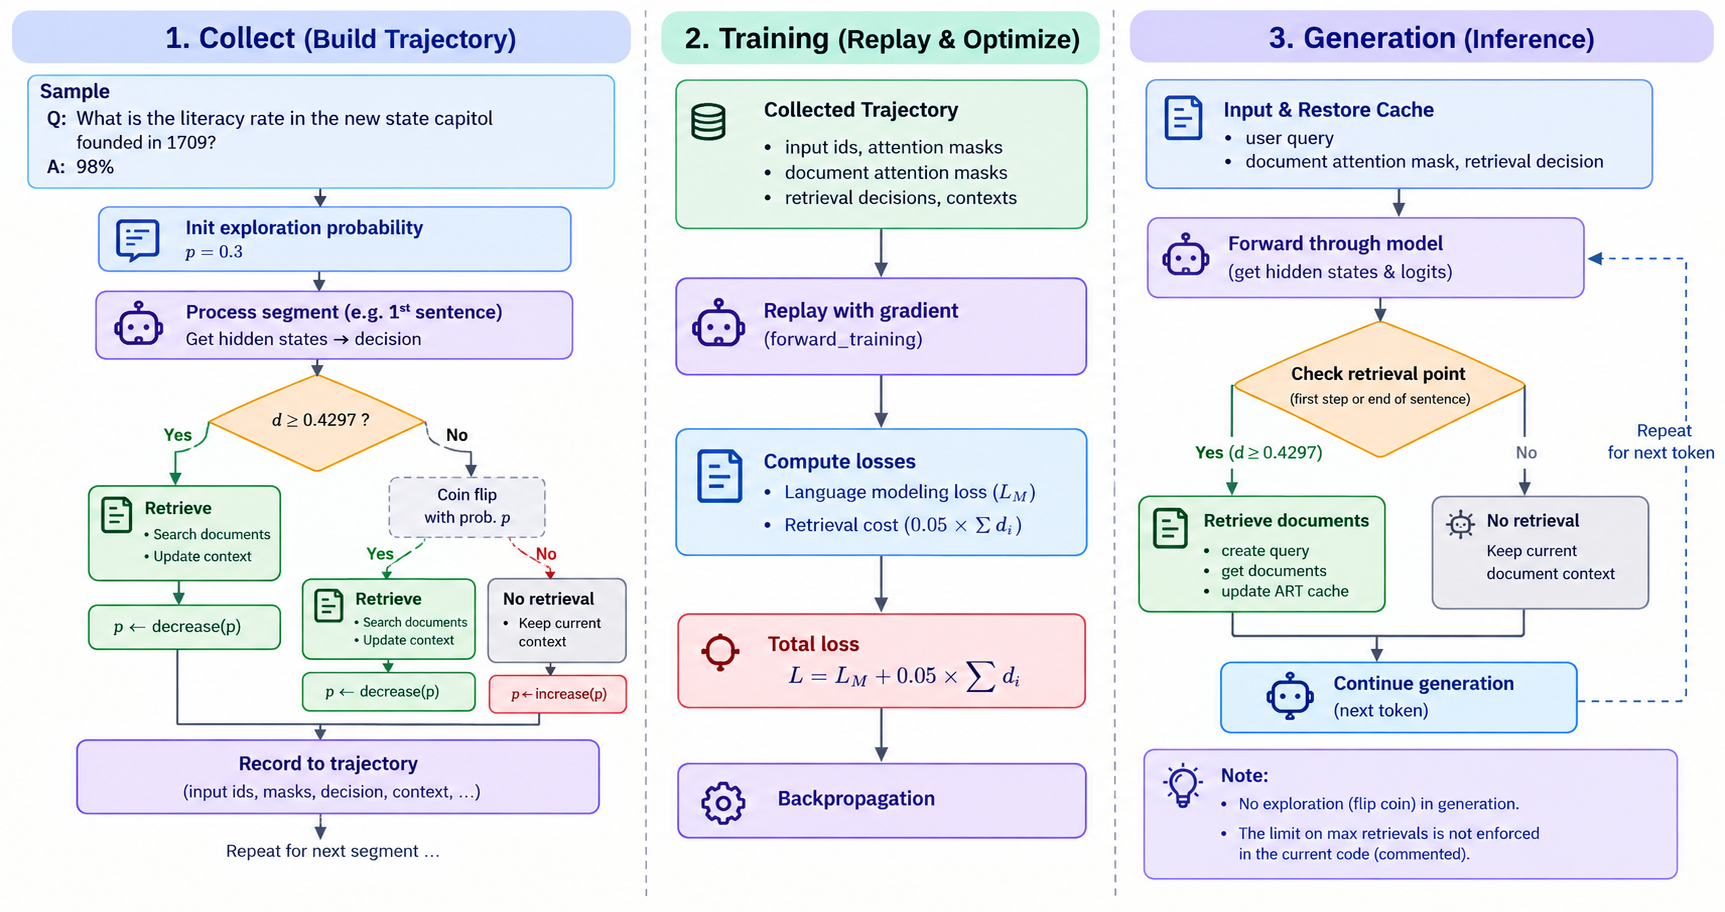
\includegraphics[
    width=\textwidth,
    height=0.82\textheight,
    keepaspectratio
]{images/ART Retrieval Workflow Diagram.png}

\end{frame}


% Slide 2 — Demo Training Configuration
\begin{frame}{Cấu hình huấn luyện Demo}

\small
\begin{itemize}
    \item \textbf{Thời gian huấn luyện:} 0.75 epoch
    \item \textbf{Các layer được huấn luyện:} 40\% layer cuối
    \item \textbf{Gradient accumulation:} 32 bước
    \item \textbf{Exploration probability ban đầu:} 0.3
    \item \textbf{Khoảng exploration probability:} 0.1--0.5
    \item \textbf{Ngưỡng quyết định (threshold):} 0.4297
\end{itemize}

\vspace{0.2cm}

\textbf{Mục tiêu:} Đánh giá mô hình demo với các mức retrieval cost và chiến lược exploration khác nhau.

\end{frame}


% Slide 3 — Demo Training 1
\begin{frame}{Demo Training 1: Retrieval Cost = 0.1}

\textbf{Chiến lược Exploration}
\begin{itemize}
    \item Tăng probability thêm 0.05, tối đa là 0.5.
    \item Giảm probability xuống mức tối thiểu là 0.1.
\end{itemize}

\vspace{0.15cm}

\textbf{Kết quả trên MuSiQue}

\centering
\begin{tabular}{lccc}
    \hline
    \textbf{Thiết lập} & \textbf{Acc} & \textbf{F1} & \textbf{EM} \\
    \hline
    Không dùng demonstration & 12.4 & 18.94 & 11.0 \\
    Có demonstration & 11.8 & 19.47 & 11.0 \\
    \hline
\end{tabular}

\vspace{0.2cm}

\small
Demonstration giúp F1 tăng nhẹ, trong khi Acc và EM không thay đổi.

\end{frame}


% Slide 4 — Demo Training 2
\begin{frame}{Demo Training 2: Retrieval Cost = 0.05}

\textbf{Chiến lược Exploration}
\begin{itemize}
    \item Tăng probability thêm 0.05, tối đa là 0.5.
    \item Giảm probability còn một nửa, nhưng không thấp hơn 0.1.
\end{itemize}

\vspace{0.15cm}

\textbf{Kết quả trên MuSiQue}

\centering
\scriptsize
\begin{tabular}{lccc}
    \hline
    \textbf{Thiết lập} & \textbf{Acc} & \textbf{F1} & \textbf{EM} \\
    \hline
    Không dùng demonstration, top-$k=3$ & 18.0 & 25.04 & 16.8 \\
    Không dùng demonstration, top-$k=5$ & 20.0 & 26.33 & 17.6 \\
    Có demonstration & 15.2 & 22.73 & 13.2 \\
    \hline
\end{tabular}

\vspace{0.2cm}

\small
Kết quả cao nhất trong thí nghiệm này đạt được khi không dùng demonstration và chọn top-$k=5$.

\end{frame}


% Slide 5 — MuSiQue Benchmark Comparison
\begin{frame}{So sánh các phương pháp trên MuSiQue}

\centering
\scriptsize
\begin{tabular}{lcc}
    \hline
    \textbf{Phương pháp} & \textbf{EM} & \textbf{F1} \\
    \hline
    No Search & 1.4 & 7.2 \\
    Vanilla RAG & 5.6 & 11.7 \\
    Iter-Retgen & 8.2 & 14.8 \\
    IRCoT & 9.2 & 17.6 \\
    Search-o1 & 4.4 & 14.0 \\
    Search-R1 & 24.4 & 32.9 \\
    R-Search & 25.8 & 34.8 \\
    R-Search-Tool & 27.2 & 36.6 \\
    \hline
ART Demo 1 (có demonstration) & 11.0 & 19.47 \\
ART Demo 2 (không demonstration, top-$k=3$) & 16.8 & 25.04 \\
\textbf{ART Demo 2 (không demonstration, top-$k=5$)} & \textbf{17.6} & \textbf{26.33} \\
    \hline
\end{tabular}

\vspace{0.2cm}

\raggedright
\tiny
Số liệu baseline lấy từ bảng so sánh đã cung cấp; số liệu ART lấy từ các thí nghiệm demo.

\end{frame}